\documentclass[tikz,border=3mm]{standalone}
\usepackage{fontspec}
\usepackage{amsmath}
\usepackage{xcolor}
\usepackage{tikz}
\usetikzlibrary{
  arrows.meta,
  backgrounds,
  calc,
  decorations.pathreplacing,
  fit,
  positioning,
  shapes.geometric,
  shapes.symbols
}

\IfFontExistsTF{Comic Sans MS}
  {\setmainfont{Comic Sans MS}}
  {\setmainfont{TeX Gyre Heros}}

\tikzset{
  >={Stealth[length=2.2mm,width=1.6mm]},
  figure title/.style={font=\fontsize{14}{16}\selectfont,align=center},
  figure subtitle/.style={font=\fontsize{8}{10}\selectfont,align=center},
  figure label/.style={font=\fontsize{7.5}{9}\selectfont,align=center},
  figure tiny/.style={font=\fontsize{6.2}{7.4}\selectfont,align=center},
  data flow/.style={-Stealth,line width=1.0pt},
  control flow/.style={-Stealth,dashed,line width=.8pt},
  projection/.style={densely dotted,line width=.8pt},
  compute/.style={rectangle,rounded corners=1.6mm,line width=.8pt,
    minimum height=.72cm,inner xsep=5pt,inner ysep=3pt,figure label},
  event/.style={diamond,aspect=1.3,line width=.8pt,inner sep=1.4pt,figure tiny},
  store/.style={cylinder,shape border rotate=90,aspect=.28,line width=.8pt,
    minimum height=.78cm,figure label},
  state/.style={circle,line width=.8pt,minimum size=.72cm,figure tiny},
  fusion/.style={regular polygon,regular polygon sides=6,line width=.8pt,
    minimum width=1.4cm,figure tiny}
}

% Derived white-paper palette for the top-conference visual research registry.
% This is a generic FigureFlow palette, not a conference or vendor brand.
\definecolor{cfink}{HTML}{1F2933}
\definecolor{cfmuted}{HTML}{667085}
\definecolor{cfdivider}{HTML}{D9E1E8}
\definecolor{cfpaper}{HTML}{FFFFFF}
\definecolor{cfnavy}{HTML}{244B6B}
\definecolor{cfblue}{HTML}{3478C9}
\definecolor{cferm}{HTML}{0E9F6E}
\definecolor{cfteal}{HTML}{087F87}
\definecolor{cfviolet}{HTML}{8064A2}
\definecolor{cfamber}{HTML}{F2B84B}
\definecolor{cfcoral}{HTML}{D9655D}
\definecolor{cfpale}{HTML}{FFF7D6}
\definecolor{cfbluebg}{HTML}{EAF2FB}
\definecolor{cftealbg}{HTML}{E8F6F1}
\definecolor{cfvioletbg}{HTML}{F1ECF7}
\definecolor{cfamberbg}{HTML}{FFF6DF}

\tikzset{
  conference panel/.style={rounded corners=2mm,draw=cfdivider,line width=.55pt,fill=cfpaper},
  conference input/.style={rounded corners=1.6mm,draw=cfnavy,fill=cfbluebg,line width=.8pt,
    minimum width=2.35cm,minimum height=.72cm,inner sep=3pt,align=center,font=\fontsize{7}{8.3}\selectfont},
  conference latent/.style={rounded corners=1.6mm,draw=cfteal,fill=cftealbg,line width=.8pt,
    minimum width=2.65cm,minimum height=.82cm,inner sep=3pt,align=center,font=\fontsize{7}{8.3}\selectfont},
  conference output/.style={rounded corners=1.6mm,draw=cfviolet,fill=cfvioletbg,line width=.8pt,
    minimum width=2.35cm,minimum height=.72cm,inner sep=3pt,align=center,font=\fontsize{7}{8.3}\selectfont},
  conference evidence/.style={rounded corners=1.2mm,draw=cfamber!80!black,fill=cfamberbg,line width=.75pt,
    minimum width=1.85cm,minimum height=.58cm,inner sep=2.2pt,align=center,font=\fontsize{6.5}{7.6}\selectfont},
  conference note/.style={rounded corners=1mm,draw=cfdivider,fill=cfpaper,line width=.5pt,
    inner sep=2pt,align=center,font=\fontsize{6.2}{7.3}\selectfont,text=cfmuted},
  conference data/.style={-Stealth,line width=1.0pt,draw=cfblue},
  conference semantic/.style={-Stealth,dashed,line width=.8pt,draw=cfamber!80!black},
  conference link/.style={densely dotted,line width=.75pt,draw=cfmuted}
}


\begin{document}
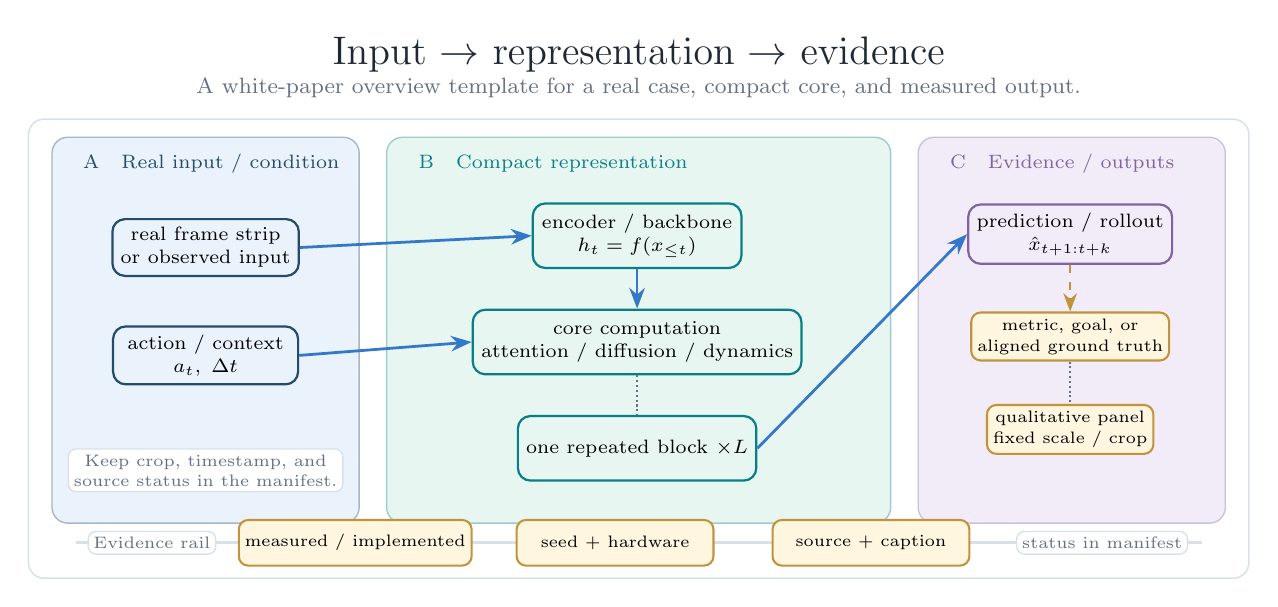
\begin{tikzpicture}[x=1cm,y=1cm]
  % A generic, editable overview distilled from hero-evidence and semantic-band
  % figures. Replace labels and evidence with paper-grounded content.
  \node[figure title,text=cfink] at (8.0,7.0)
    {Input $\rightarrow$ representation $\rightarrow$ evidence};
  \node[figure subtitle,text=cfmuted] at (8.0,6.58)
    {A white-paper overview template for a real case, compact core, and measured output.};

  \begin{scope}[on background layer]
    \fill[conference panel] (.25,.35) rectangle (15.75,6.18);
    \fill[rounded corners=2mm,fill=cfbluebg,draw=cfnavy!40,line width=.5pt]
      (.55,1.05) rectangle (4.45,5.95);
    \fill[rounded corners=2mm,fill=cftealbg,draw=cfteal!40,line width=.5pt]
      (4.80,1.05) rectangle (11.20,5.95);
    \fill[rounded corners=2mm,fill=cfvioletbg,draw=cfviolet!40,line width=.5pt]
      (11.55,1.05) rectangle (15.45,5.95);
  \end{scope}

  \node[figure label,anchor=west,text=cfnavy] at (.82,5.62) {A\quad Real input / condition};
  \node[figure label,anchor=west,text=cfteal] at (5.08,5.62) {B\quad Compact representation};
  \node[figure label,anchor=west,text=cfviolet] at (11.83,5.62) {C\quad Evidence / outputs};

  \node[conference input] (frame) at (2.50,4.55) {real frame strip\\or observed input};
  \node[conference input] (action) at (2.50,3.18) {action / context\\$a_t,\;\Delta t$};
  \node[conference note] at (2.50,1.72) {Keep crop, timestamp, and\\source status in the manifest.};

  \node[conference latent] (encoder) at (7.98,4.70) {encoder / backbone\\$h_t = f(x_{\le t})$};
  \node[conference latent] (core) at (7.98,3.35) {core computation\\attention / diffusion / dynamics};
  \node[conference latent] (repeat) at (7.98,2.00) {one repeated block $\times L$};
  \draw[conference data] (frame.east) -- (encoder.west);
  \draw[conference data] (action.east) -- (core.west);
  \draw[conference data] (encoder) -- (core);
  \draw[conference link] (core) -- (repeat);

  \node[conference output] (prediction) at (13.48,4.72) {prediction / rollout\\$\hat{x}_{t+1:t+k}$};
  \node[conference evidence] (metric) at (13.48,3.42) {metric, goal, or\\aligned ground truth};
  \node[conference evidence] (qual) at (13.48,2.24) {qualitative panel\\fixed scale / crop};
  \draw[conference data] (repeat.east) -- (prediction.west);
  \draw[conference semantic] (prediction) -- (metric);
  \draw[conference link] (metric) -- (qual);

  % The lower rail is intentionally sparse: it encodes provenance/measurement,
  % not decorative marketing claims.
  \draw[draw=cfdivider,line width=1.0pt] (.85,.80) -- (15.15,.80);
  \node[conference note,anchor=west] at (1.0,.80) {Evidence rail};
  \node[conference evidence,minimum width=2.6cm] at (4.40,.80) {measured / implemented};
  \node[conference evidence,minimum width=2.5cm] at (7.70,.80) {seed + hardware};
  \node[conference evidence,minimum width=2.5cm] at (10.95,.80) {source + caption};
  \node[conference note,anchor=east] at (14.98,.80) {status in manifest};
\end{tikzpicture}
\end{document}
